\documentclass{beamer}
\usetheme{Boadilla}
\usepackage[T1]{fontenc}

\title{Redundantny system plików}

\author{Kacper Pieniążek}
\date{\today}

\begin{document}
	\begin{frame}
		\titlepage
	\end{frame}

	\section{Section 1}
	\subsection{sub a}
	
	\begin{frame}
		\frametitle{Cel pracy}
		\begin{itemize}
			\item System plików zapewniający ochronę danych nawet w przypadku ich uszkodzenia.
			\item W oparciu o interfejs FUSE.
		\end{itemize}
		
	\end{frame}

	\begin{frame}
		\frametitle{Założenia pracy}
		\begin{itemize}
			\pause
			\item Wykrywanie niezgodności danych
				\begin{itemize}
					\item Sumy kontrolne
					\item Kody korekcyjne
				\end{itemize}
			\pause
			\item Odzyskiwanie danych
			\begin{itemize}
				\item Duplikacja danych
				\item Kody korekcyjne
			\end{itemize}
			\pause
			\item Obsługa wybranych funkcjonalności systemu plików
			\pause
			\item Wygodne użytkowanie
			\begin{itemize}
				\item Podział i duplikacja danych jak najbardziej transparentna dla użytkownika
				\item Rozwiązywanie konfliktów w przypadku niezgodności danych
				\item Dostosowanie systemu do własnych potrzeb
			\end{itemize}
		\end{itemize}
	\end{frame}
	
	\begin{frame}
		\frametitle{Analiza problemu}

		\begin{itemize}
			\item Jak zapewnić redundancję?
			\pause
			\item Jak zapewnić spójność danych?
			\begin{itemize}
				\item W przypadku braku synchronizacji między replikami, wybór poprawnych danych
			\end{itemize}
			\pause
			\item Jak wykrywać rozbieżność danych?
			\begin{itemize}
				\item Podczas operowania na uszkodzonych danych; błędny odczyt, kody korekcyjne, sumy kontrolne 
			\end{itemize}
			\pause
			\item Jak naprawiać rozbieżność danych?
			
		\end{itemize}
	\end{frame}
		
	\begin{frame}
		\frametitle{Rozwiązanie}
			\begin{block}{Definicja}
				Replika - jeden z podsystemów zawierający kopię chronionych danych
			\end{block}
			\pause
			\begin{itemize}
				\item Cały system może być podzielony na warstwy współpracujące ze sobą. 
				\begin{itemize}
					\item Każdy typ repliki to nowa warstwa
				\end{itemize}
				\pause
				\item Podział na warstwy umożliwia rozwiązania typu RAID
			\end{itemize}
			
	\end{frame}

		
\begin{frame}
	\frametitle{Rozwiązanie}
	\begin{block}{Definicja}
		Replika duplikująca kopiuje chronione dane bez dodatkowych informacji
	\end{block}
	\pause
	\begin{block}{Definicja}
		Replika blokowa rozdziela chronione dane na bloki zależne od wybranej implementacji; Może zawierać dodatkowe informacje potrzebne w przypadku uszkodzenia
	\end{block}
\end{frame}

\begin{frame}
	\frametitle{Replika typu 0}
		\begin{columns}
		\column{0.7\textwidth}
		Lorem ipsum
		\column{0.3\textwidth}
		\begin{figure}
			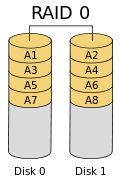
\includegraphics[scale=0.5]{raid-0.png}
		\end{figure}
		\end{columns}
\end{frame}
	
\begin{frame}
	\frametitle{Replika typu 1}
	\begin{columns}
		\column{0.7\textwidth}
		Lorem ipsum
		\column{0.3\textwidth}
		\begin{figure}
			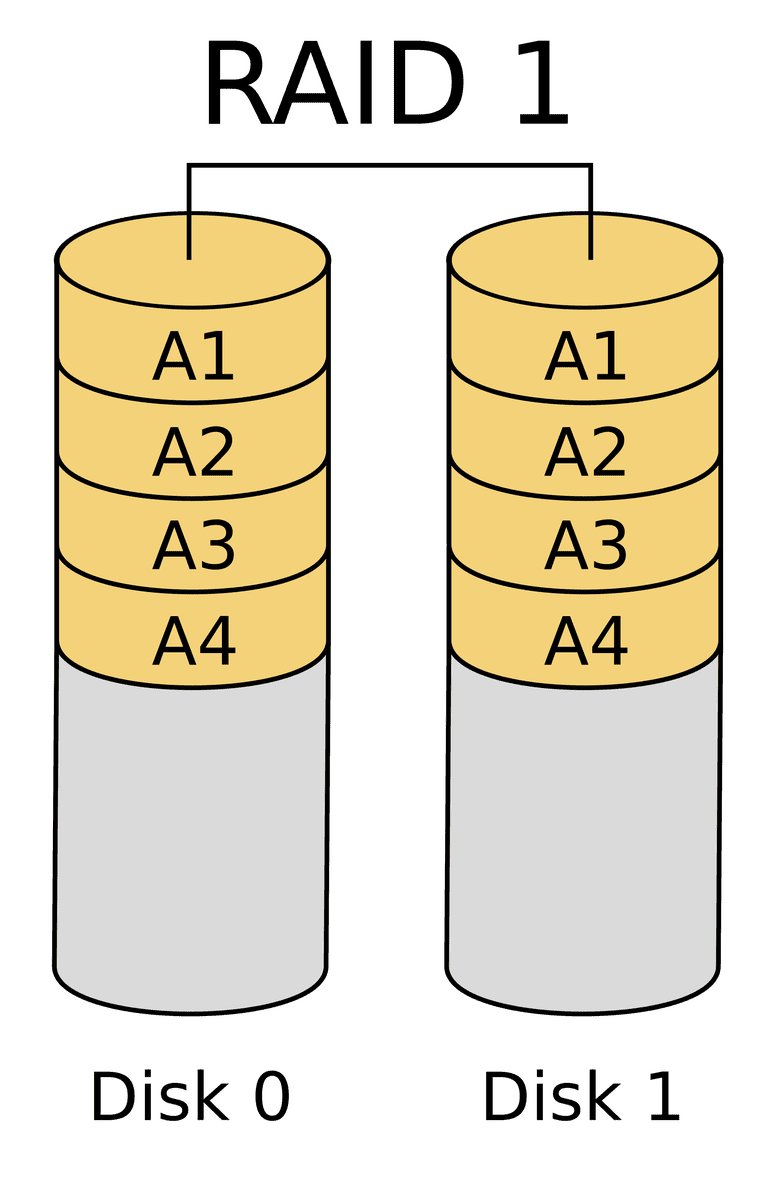
\includegraphics[scale=0.09]{raid-1.png}
		\end{figure}
	\end{columns}
\end{frame}
	
\begin{frame}
	\frametitle{Replika typu 2}
	\begin{columns}
		\column{0.4\textwidth}
		Lorem ipsum
		\column{0.6\textwidth}
		\begin{figure}
			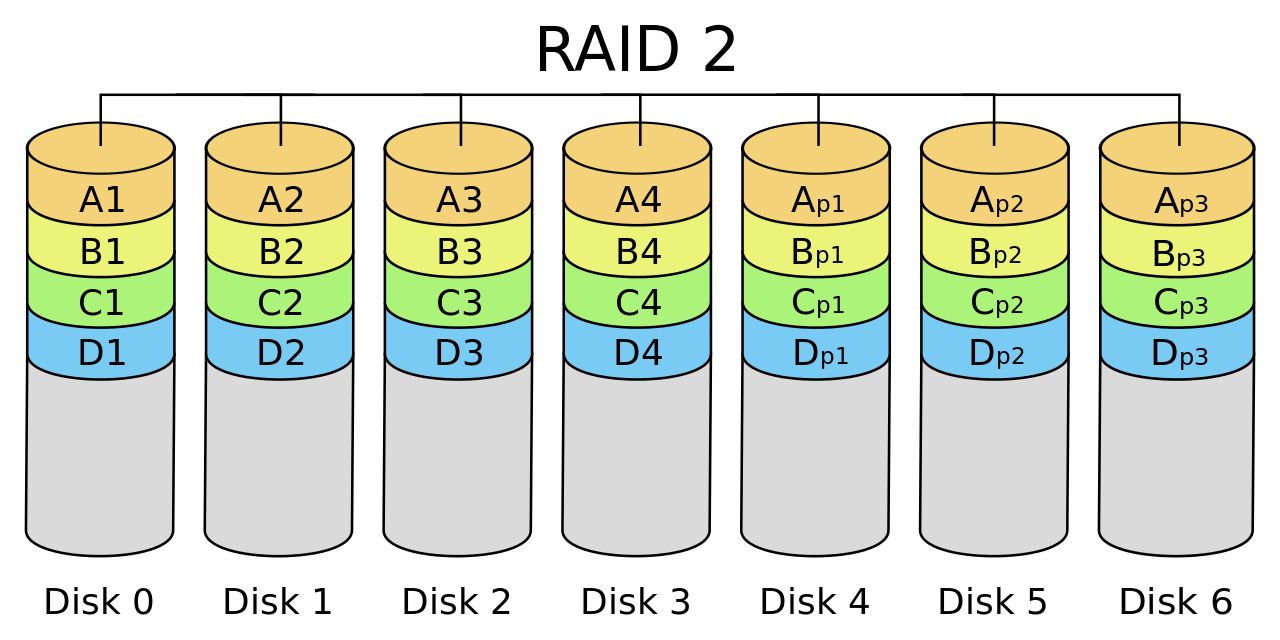
\includegraphics[scale=0.1]{raid-2.png}
		\end{figure}
	\end{columns}
\end{frame}
			
\begin{frame}
	\frametitle{Replika typu 3}
	\begin{columns}
		\column{0.4\textwidth}
		Lorem ipsum
		\column{0.6\textwidth}
		\begin{figure}
			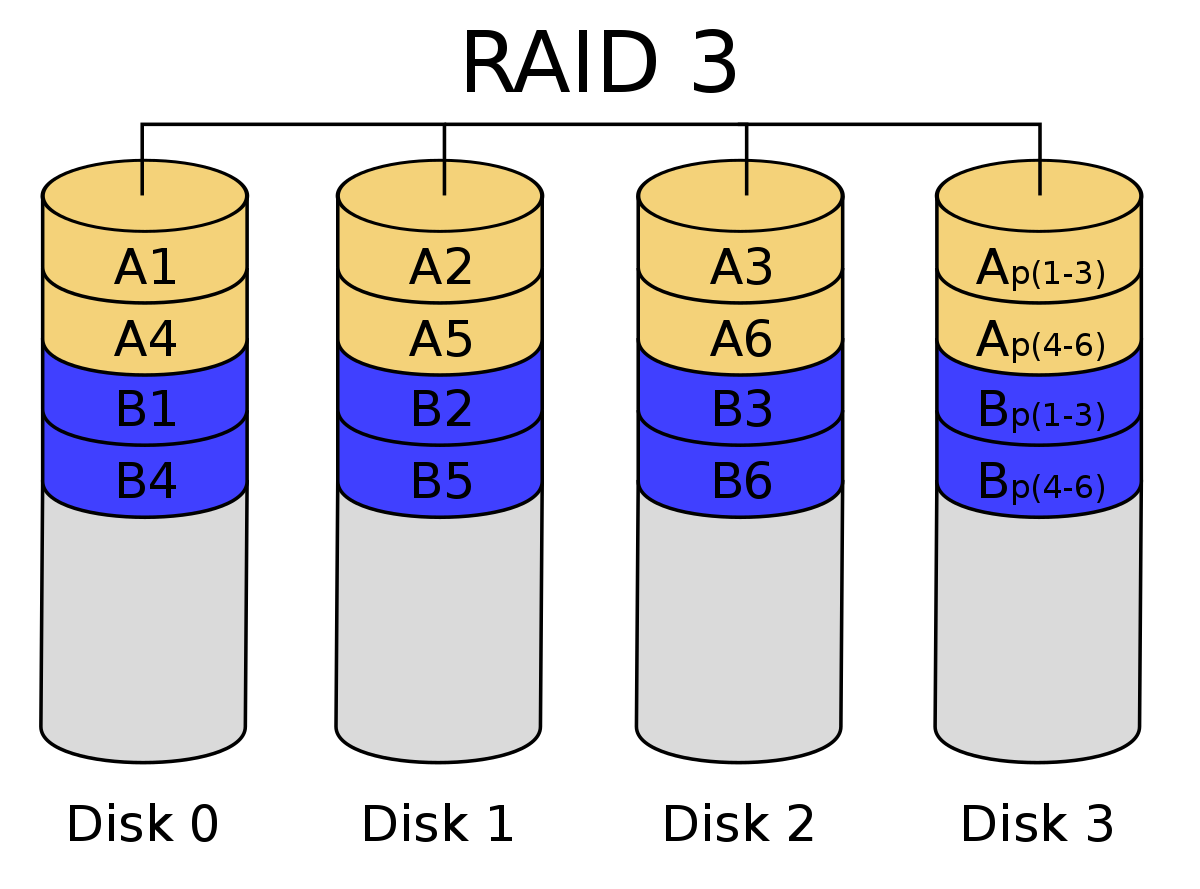
\includegraphics[scale=0.1]{raid-3.png}
		\end{figure}
	\end{columns}
\end{frame}

\begin{frame}
	\frametitle{Replika typu 4}
	\begin{columns}
		\column{0.4\textwidth}
		Lorem ipsum
		\column{0.6\textwidth}
		\begin{figure}
			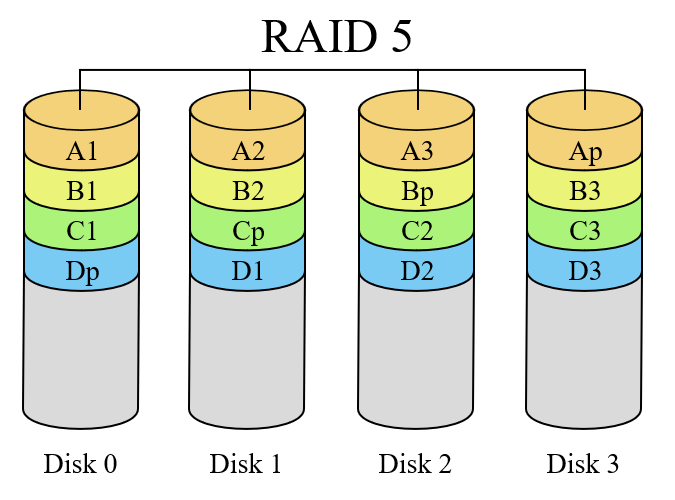
\includegraphics[scale=0.2]{raid-5.png}
		\end{figure}
	\end{columns}
\end{frame}
		
	\begin{frame}
		\frametitle{Przykłady}
		\begin{block}{Przykład}
			Dysk, na którym zamontowana była jedna z replik duplikujących dane został odłączony. 
		\end{block}
		\pause
		\begin{block}{Przykład}
			Wystąpił błąd poczas zapisu do jednej z replik blokowych.
		\end{block}
		\pause
		\begin{block}{Przykład}
			Obrócone bity na danych w jednej z replik.
		\end{block}
	\end{frame}
	
	\begin{frame}
		\frametitle{Konfiguracja oraz komunikacja}

	\end{frame}

\end{document}